\subsection{Election November 2, 2004: *Bush vs Kerry}
\begin{frame}[t]{Election November 2, 2004: *George W Bush}
\small

\begin{columns}[T, onlytextwidth]
\column{0.48\textwidth}
\vspace{-1em}
{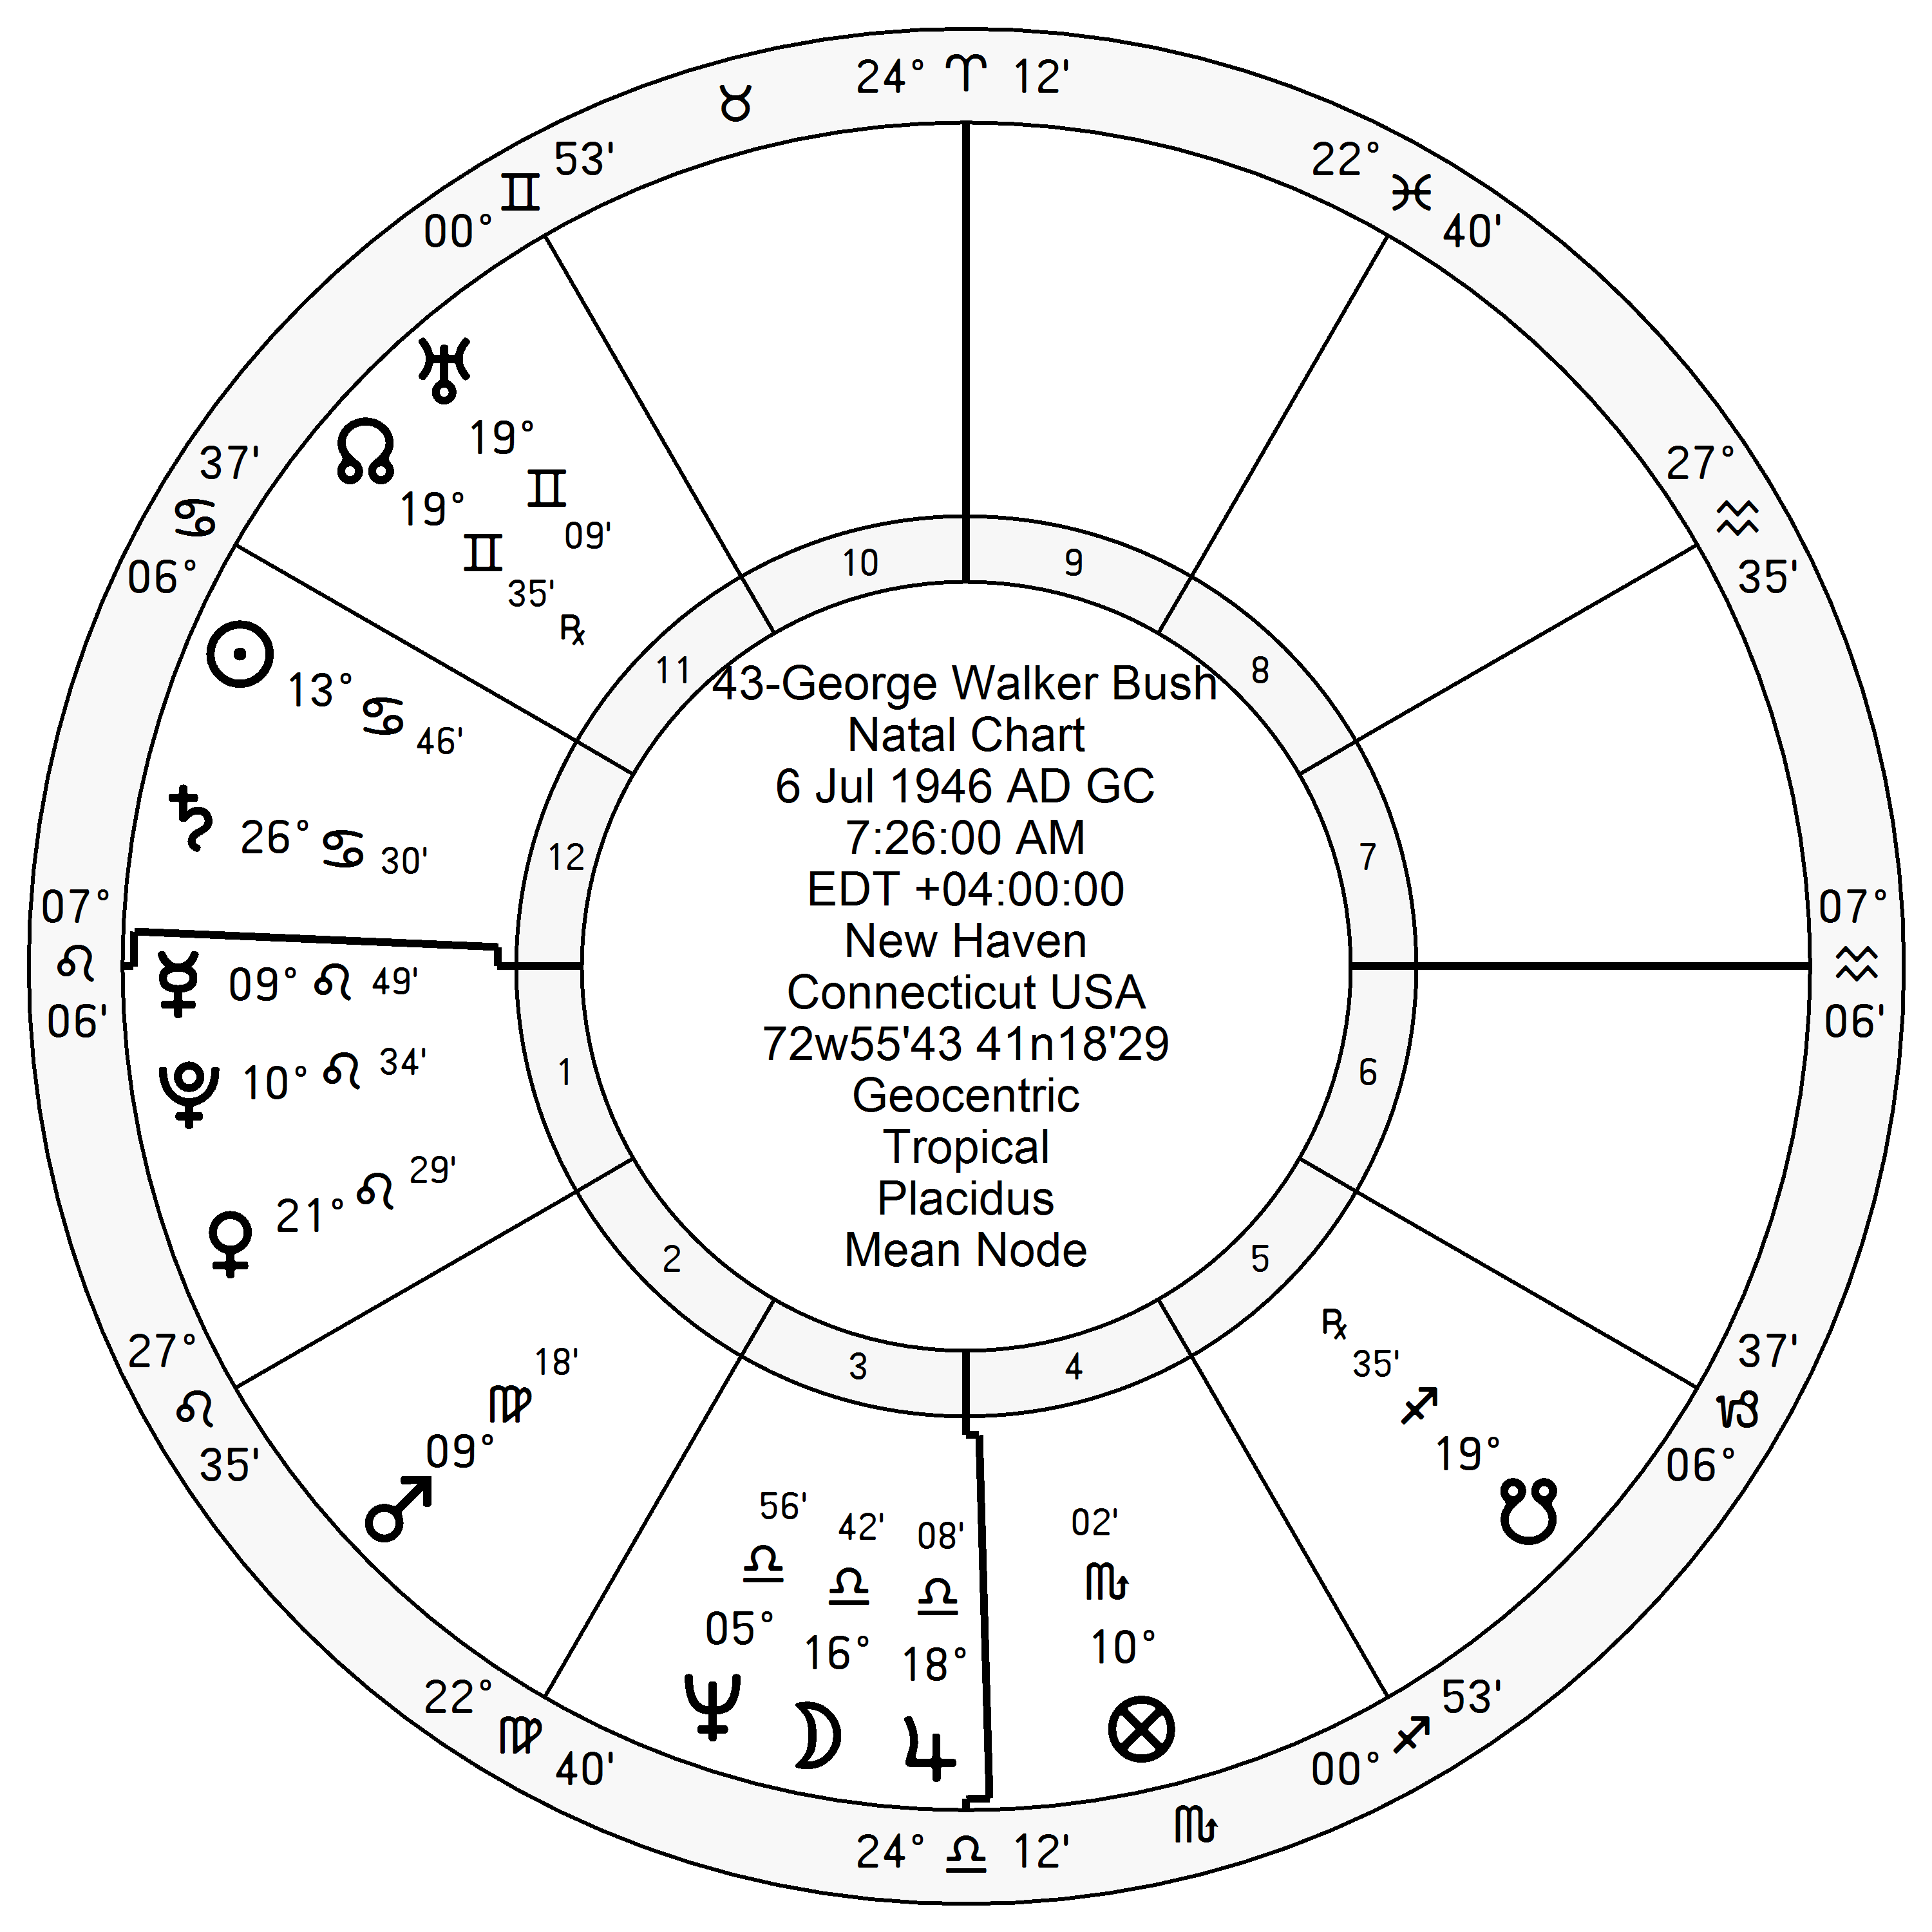
\includegraphics[width=0.9\textwidth]{charts/GW-Bush.png}}
\fontsize{7pt}{8pt}\selectfont

\Mercury\, \Sextile\, P1; in N1 \Square\, N10 \\
\Jupiter\, \Trine\, P1; in mitigated \Quincunx\, (\Opposition) N10

\column{0.48\textwidth}
\vspace{-1em}
{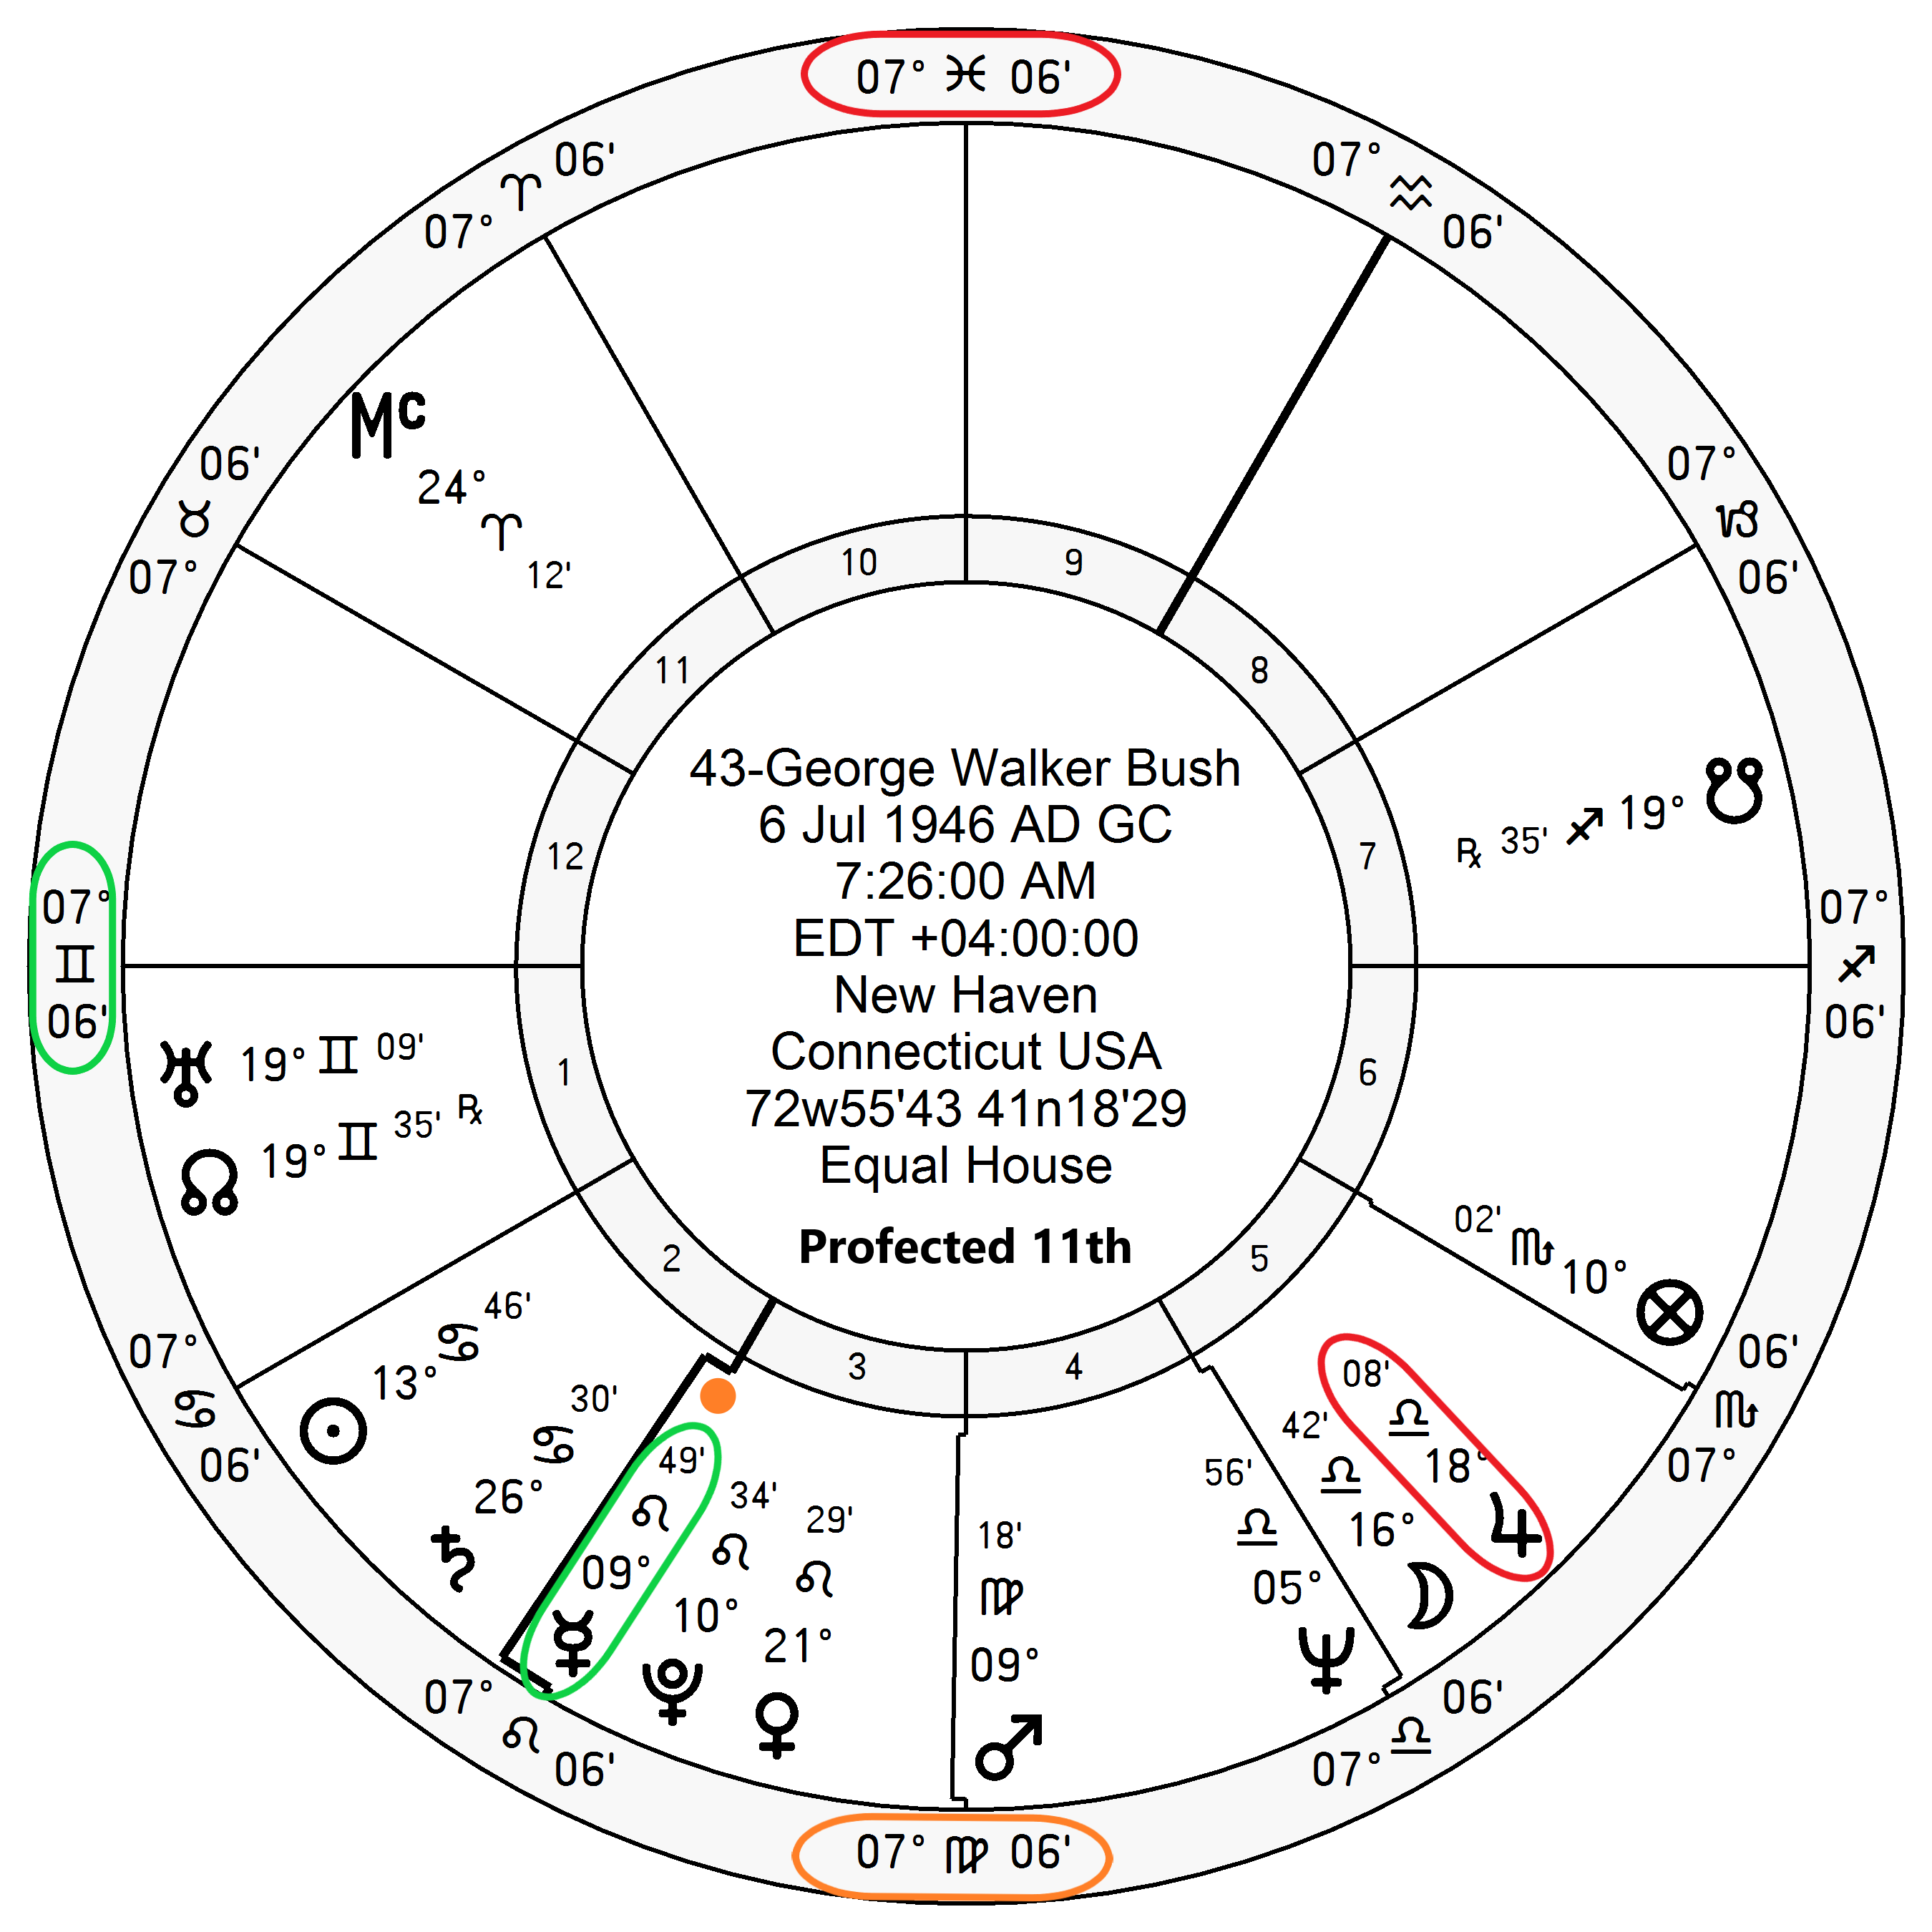
\includegraphics[width=0.9\textwidth]{charts/GW-Bush-Prof-11th.png}}
\fontsize{8pt}{9pt}\selectfont

\textbf{\dgreen P1}=N11
	$\Rightarrow$ \Mercury\, $\Rightarrow$ \textbf{\dgreen P3/N1}\\
\textbf{\red P10}=N9
	$\Rightarrow$ \Jupiter\, $\Rightarrow$ P5/\textbf{\dgreen N3}\\
PE=P4/\textbf{\dgreen N3}
	 $\Rightarrow$ \Mercury\, $\Rightarrow$ \textbf{\dgreen P3/N1}

\end{columns}
\end{frame}

% ===================================================
\begin{frame}[t]{Election November 2, 2004: John Kerry}
\small
\begin{columns}[T, onlytextwidth]
\column{0.48\textwidth}
\vspace{-1em}
{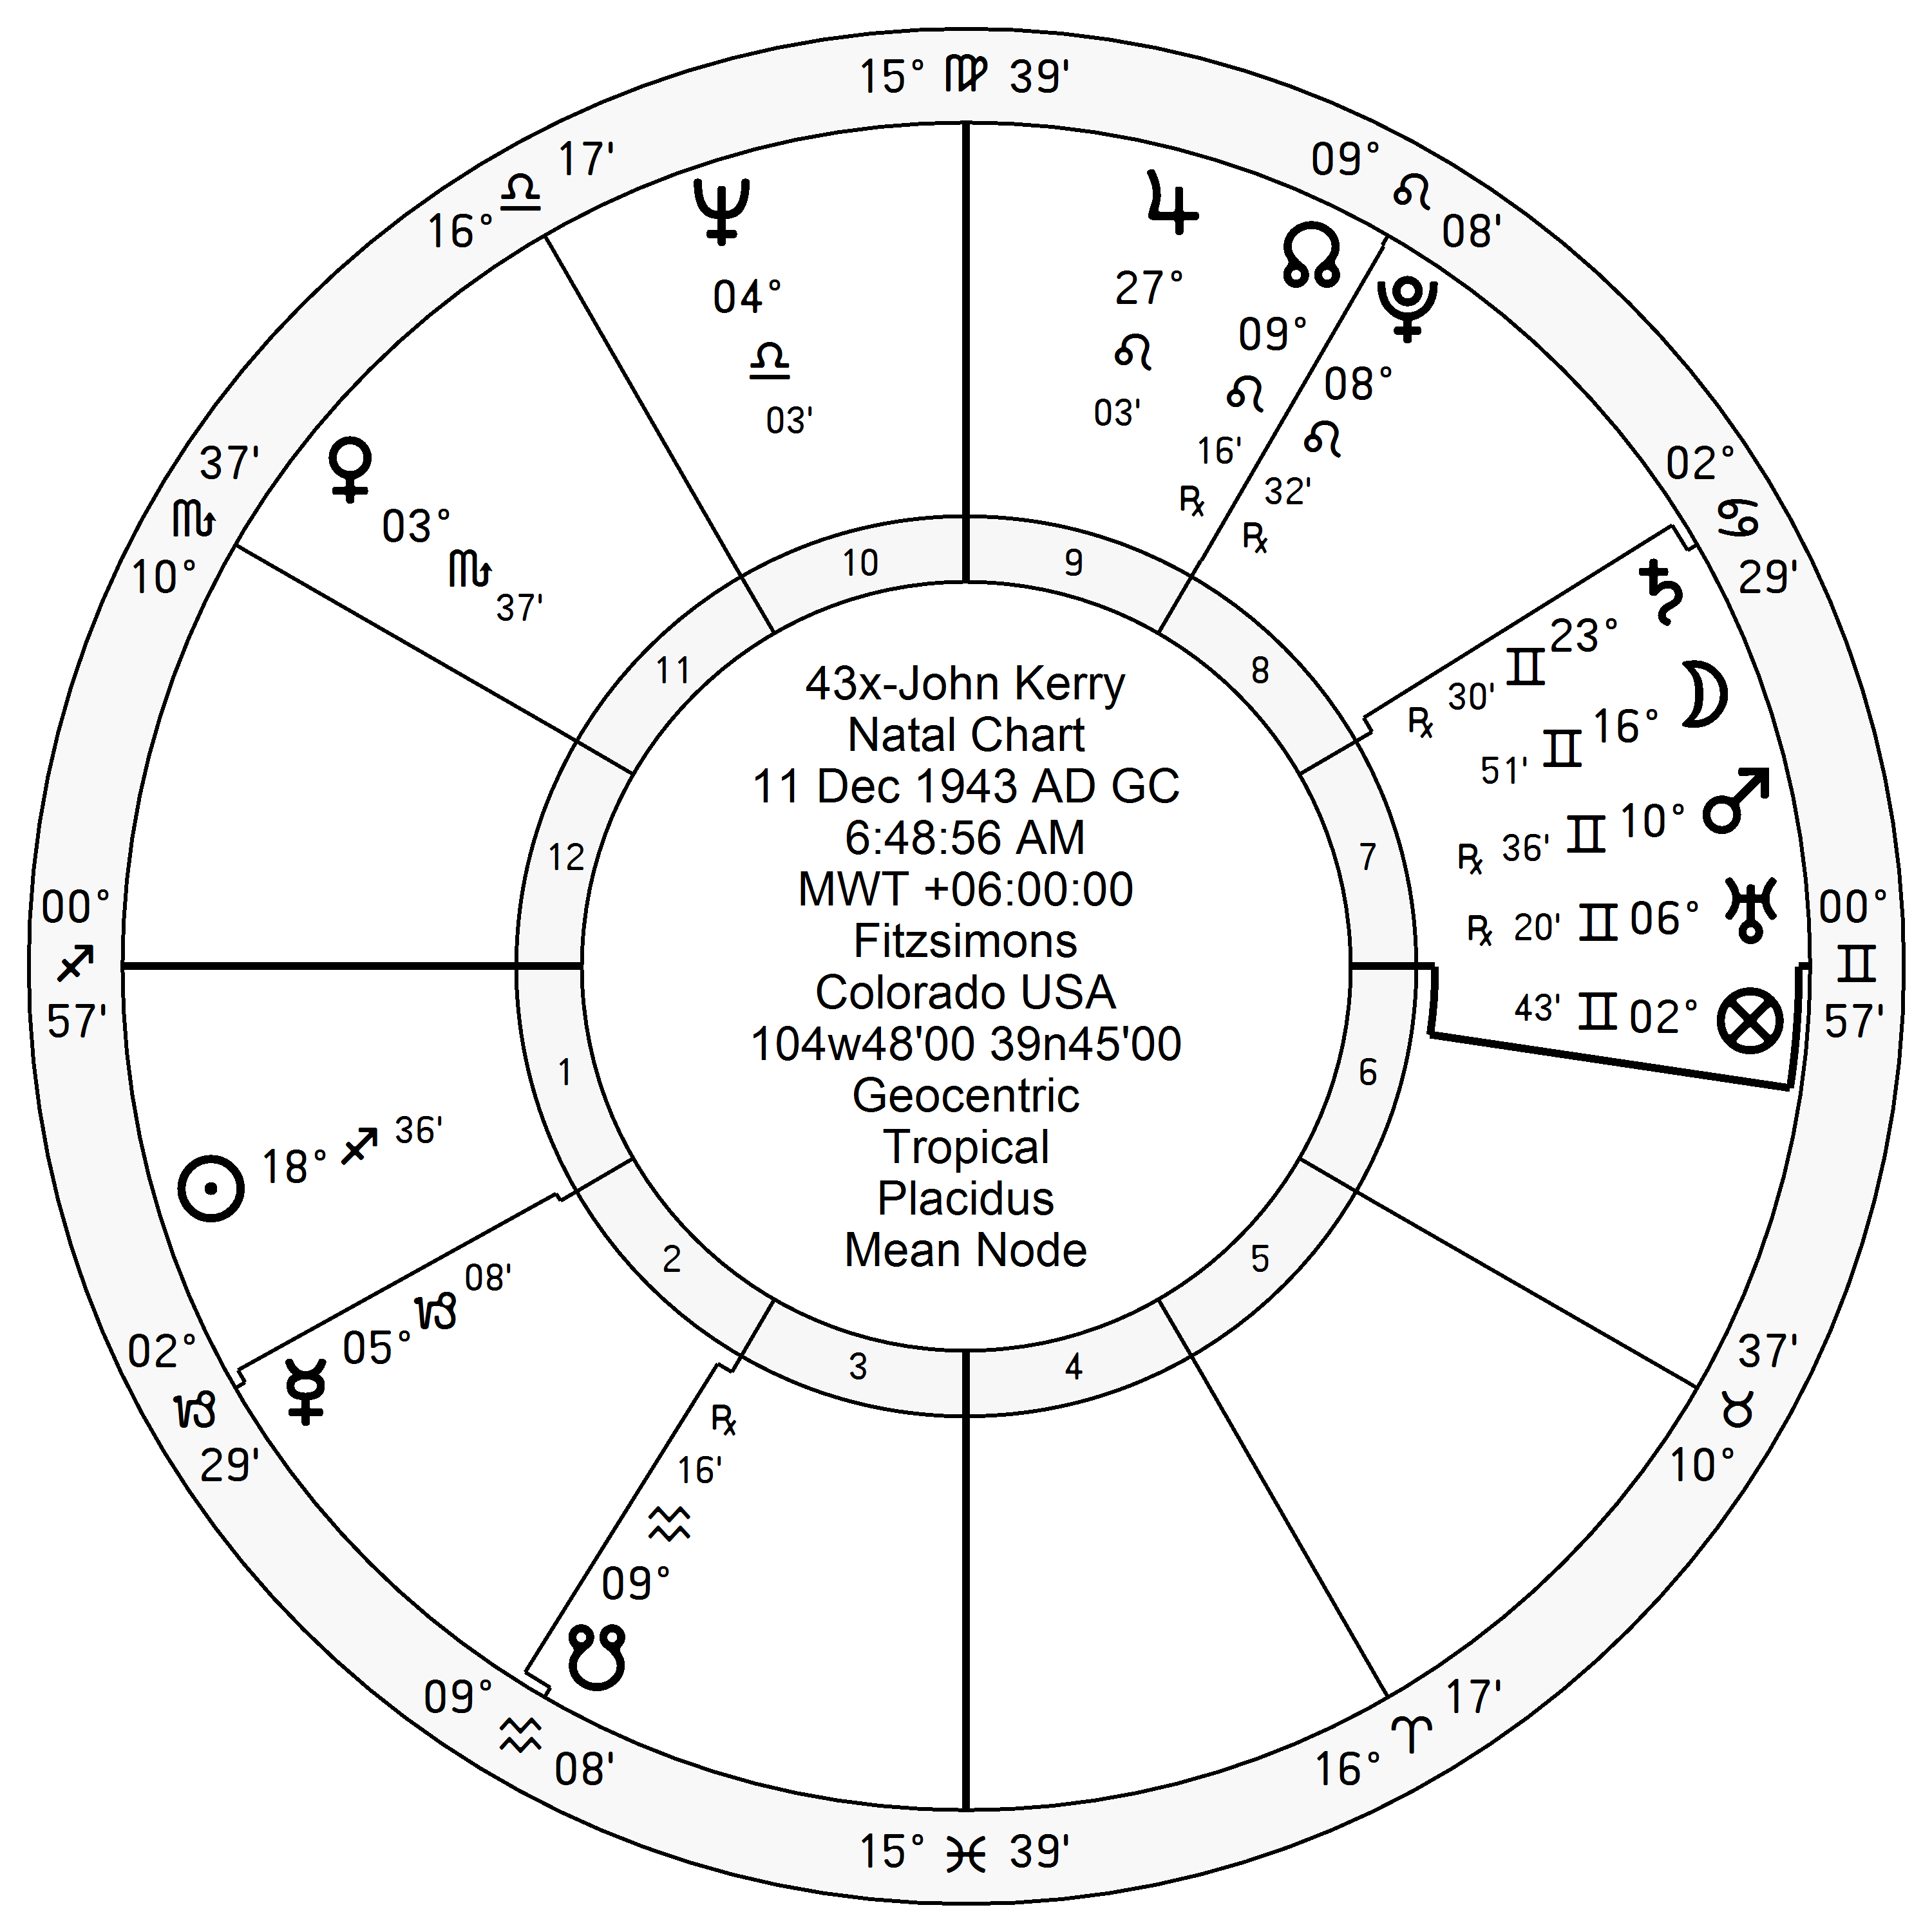
\includegraphics[width=0.9\textwidth]{charts/Kerry.png}}
\fontsize{7pt}{8pt}\selectfont

Kerry's birth time is out of scope for the original study; the chart is based on Starkman's rectified time as given on Astrodatabank.\\
\vspace{0.5em}
\Jupiter\, \Trine\, P1, N1 \\
\Mercury\, \Trine\, P10, N10 \\
\Venus\, \Sextile\, P10

\column{0.48\textwidth}
\vspace{-1em}
{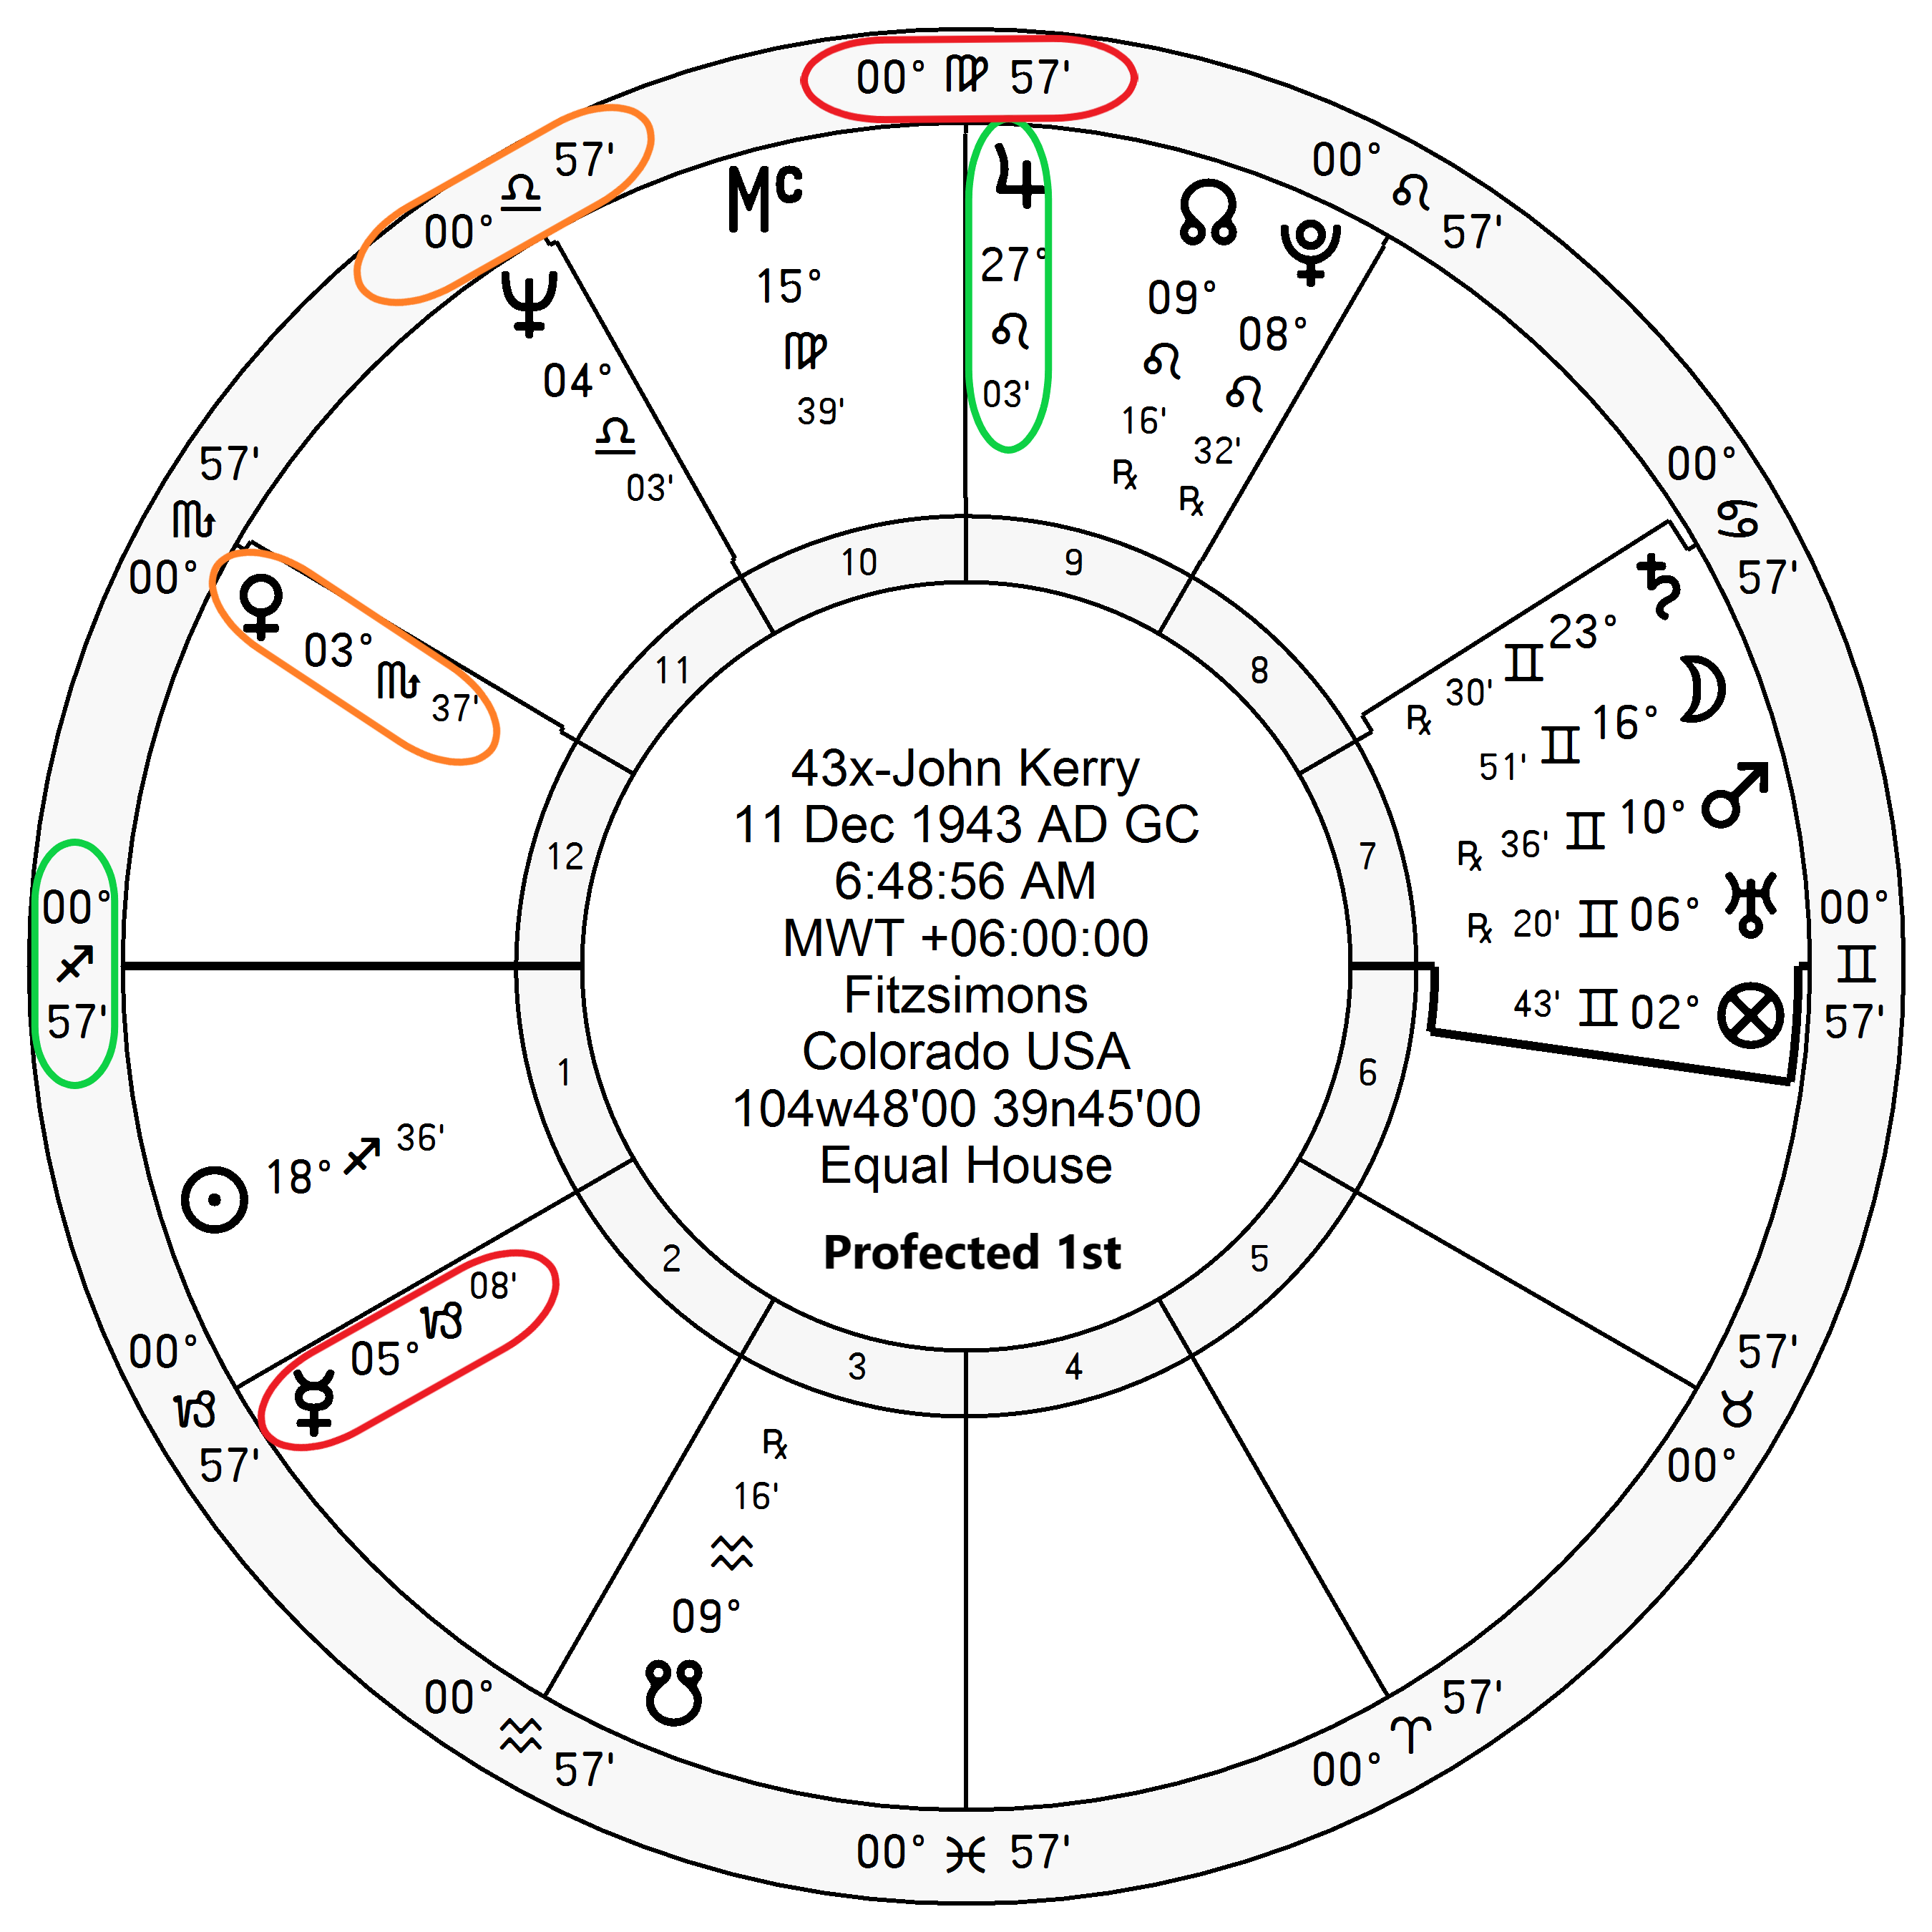
\includegraphics[width=0.9\textwidth]{charts/Kerry-Prof-1st.png}}
\fontsize{8pt}{9pt}\selectfont
\textbf{\dgreen P1}=N1
	$\Rightarrow$ \Jupiter\, $\Rightarrow$ P9/N9\\
\textbf{\red P10}=N10
	$\Rightarrow$ \Mercury\, $\Rightarrow$ P2/N2\\
PE=P11/N11
	 $\Rightarrow$ \Venus\, $\Rightarrow$ P12/N11

\end{columns}
\end{frame}
